\documentclass[11pt]{article}
\usepackage[utf8]{inputenc}
\usepackage[T1]{fontenc}
\usepackage{tikz}
\usetikzlibrary{positioning,calc}
% El estilo de las figuras vive en su propio archivo (es el `stampFiles` del cache): cambiarlo cambia el sello.
% Estilo de las figuras: es el archivo de sello (`figureCache.stampFiles`). Cualquier cambio acá cambia el nombre de todas.
\tikzset{miestilo/.style={thick,blue!60!black}}


\begin{document}

\section{Principal}

Una figura en el archivo raíz, dentro de \texttt{figure}.

\begin{figure}[ht]
  \centering
  
\begin{tikzpicture}
    \draw[miestilo] (0,0) circle (1);
  \end{tikzpicture}
  \caption{Un círculo.}
\end{figure}

\section{Capítulo A}

Dos figuras en un archivo que entra por \texttt{\textbackslash input}.

\begin{figure}[ht]
  \centering
  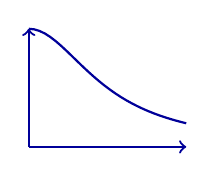
\begin{tikzpicture}
    \draw[miestilo,->] (0,0) -- (2,0);
    \draw[miestilo,->] (0,0) -- (0,1.5);
    \draw[miestilo,domain=0:2,samples=30] plot (\x,{1.5/(1+\x*\x)});
  \end{tikzpicture}
  \caption{Una curva.}
\end{figure}

\begin{figure}[ht]
  \centering
  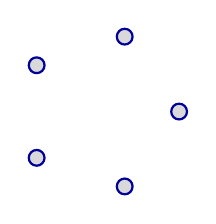
\begin{tikzpicture}
    \foreach \k in {0,...,4} {
      \draw[miestilo,fill=gray!30] ({cos(72*\k)},{sin(72*\k)}) circle (0.1);
    }
  \end{tikzpicture}
  \caption{Cinco puntos.}
\end{figure}

\section{Capítulo B}

Una figura en un archivo que entra por \texttt{\textbackslash include}, dentro de una subcarpeta.

\begin{figure}[ht]
  \centering
  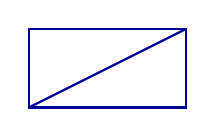
\begin{tikzpicture}
    \draw[miestilo] (0,0) rectangle (2,1);
    \draw[miestilo] (0,0) -- (2,1);
  \end{tikzpicture}
  \caption{Un rectángulo.}
\end{figure}


Un \texttt{tikzpicture} \emph{fuera} de \texttt{figure}, con \texttt{remember picture, overlay}, como los íconos del template.

\begin{tikzpicture}[remember picture,overlay]
  \node[anchor=north east,red] at (current page.north east) {marca de agua};
\end{tikzpicture}

\end{document}
